\documentclass[11pt]{article}
\usepackage[francais]{babel}
\usepackage[utf8]{inputenc}
\usepackage[T1]{fontenc}
\usepackage{graphicx}

\graphicspath{{Graphiques/}}

\begin{document}

\title{\textbf{Synthèse article ADA} \\Dynamic Warp Formation and Scheduling for Efficient GPU Control Flow
}
\author{Olivier Pelgrin}
%\tableofcontents

%\newpage

\maketitle

\section{Introduction}

Ces dernières décennies, le développement de jeux vidéos graphiquement complexes en 3-dimensions a conduit à l'élaboration de processeurs spécialisés dans le calcul d'images en 3D.
\\En effet pour répondre à la complexité croissante de graphismes des jeux vidéos, le développement d'accélérateurs spécialisés a été nécessaire pour offrir le niveau de performance requis.
\\Ces processeur spécialisés sont appelés GPUs (Graphics Processing Units).
\\Au fil des années, et pour répondre aux nouveaux besoins des jeux vidéos, les GPUs sont devenus de plus en plus flexibles, devenant programmables, remplaçant une large partie de leur fonctions fixes par des programmes \emph{shaders} écrits par les développeurs d'applications.
\\Depuis plus d'une dizaine d'année, les GPUs sont devenus \emph{turing-complet} ouvrant la voie à de nouvelles utilisations, autres que le jeux vidéo.
Les GPUs sont depuis devenus très utilisée pour le calcul scientifique grâce à l'apparition d'APIs de calcul généralistes (comme CUDA et OpenCL par exemple), permettant la programmation des GPUs en dehors du contexte des jeux vidéos.

\newpage

\section{Contexte et problématique}

\subsection{Architecture des GPUs}

A l'origine, les tâches pour lesquels les GPUs ont été créés sont hautement parallélisable par nature (opérations par pixel/vertex), ce qui fait que les GPUs sont des architectures très parallèles.
\\Pour réduire la complexité des flux de contrôle, la plupart des architectures GPUs utilisent des pipelines single-instruction multiple-data (SIMD). Cela permet un haut niveau de parallélisme pour un coût relativement faible.

Le plus souvent, les GPUs groupent ensemble des threads exécutant le même programme dans des \emph{warps}. Tous les threads d'un warp s'exécutent de manière synchronisée sur un pipeline SIMD du GPU.
Tous les threads exécutent exactement la même instruction en même temps, mais sur des données différentes.

\subsection{Problématique des flux de contrôle}

Pendant longtemps, cette approche a eu de très bon résultats sur les \emph{shaders} des jeux vidéos. En effet, historiquement, ces shaders sont pauvres en opérations de contrôle, ce qui permet aux warps de s'exécuter du début à la fin de manière synchronisée.
\\Lors d'opérations de contrôle, il est possible que les threads d'un warp ne peuvent s'exécuter de manière synchronisée, par exemple si des threads prennent une branche différente lors d'un branchement.
Dans ce cas, il faut exécuter chaque partie du branchement séparément, ce qui peut amener à une sous utilisation du pipeline SIMD, avec seulement un faible nombre de threads s'exécutant simultanément.

\begin{figure}[h]
   \caption{\label{IPC} Perte de performance lié aux branchements sur des architectures SIMD}
   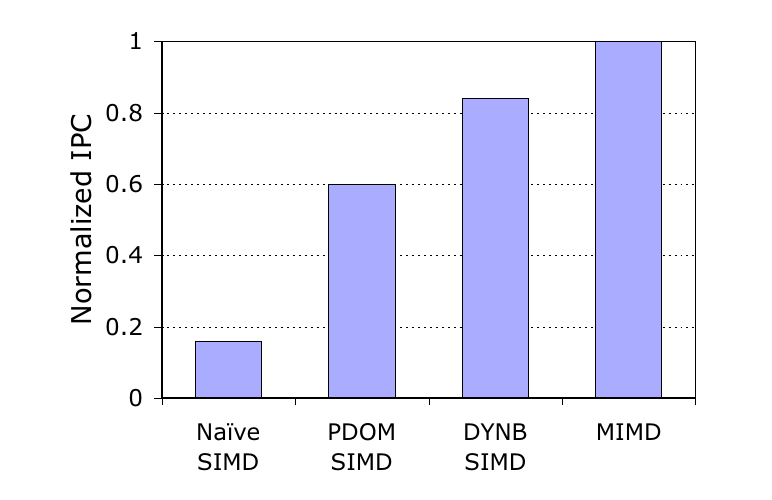
\includegraphics[scale=.6]{ipc}
\end{figure}

Sur la figure~\ref{IPC}, on peut observer la perte de performance due aux branchements à l'exécution de threads SPMD sur des architectures SIMD.

La divergence de branchements au sein d'un warp était à l'époque de la publication de l'article (2007) encore assez peu problématique dans le cadre de shaders de jeu vidéo (ce qui est moins vrai maintenant en 2017). Cependant les applications de calcul généralistes sur GPUs souffraient déjà de ce problème.
\\Les auteurs de l'article proposent plusieurs mécanismes permettant de réduire significativement l'impact des branchements divergeant sur les architectures SIMD des GPUs.


\section{Solutions proposées}

La façon naïve de gérer la divergence de branchements au sein d'un warp consiste à sérialiser l'exécution des threads.
Cette méthode est facile à implémenter et permet de gérer la divergence.
Cependant, il est possible que les threads continuent de diverger lors de branchements divergeant successifs. Il ainsi possible de se retrouver dans une situation où tous les threads d'un warp sont isolés des autres, et s'exécutent les uns après les autres sur le pipeline SIMD.
De manière évidente, une telle solution est inacceptable sur le plan des performances, ce montre le besoin de solutions plus efficaces pour gérer les branchements.

Dans leur article, les auteurs font plusieurs propositions, la première est un mécanisme de convergence des threads dès que possible après un (des) branchements divergeant.

\subsection{Convergence}

Cette première solution consiste à faire converger dès que possible des threads ayant divergés pour les resynchroniser lorsqu'ils se retrouvent à nouveau sur le même flux de contrôle.
L'intérêt est notamment d'empêcher les threads de trop diverger en repérant les points de convergence pour recommencer une exécution synchronisée quand c'est possible.
\\Lors de la détection d'un branchement divergeant, le mécanisme repère le moment où les threads convergent afin de resynchroniser les threads à ce point.

\begin{figure}[h]
   \caption{\label{BRANCHE} Illustration du mécanisme de convergence}
   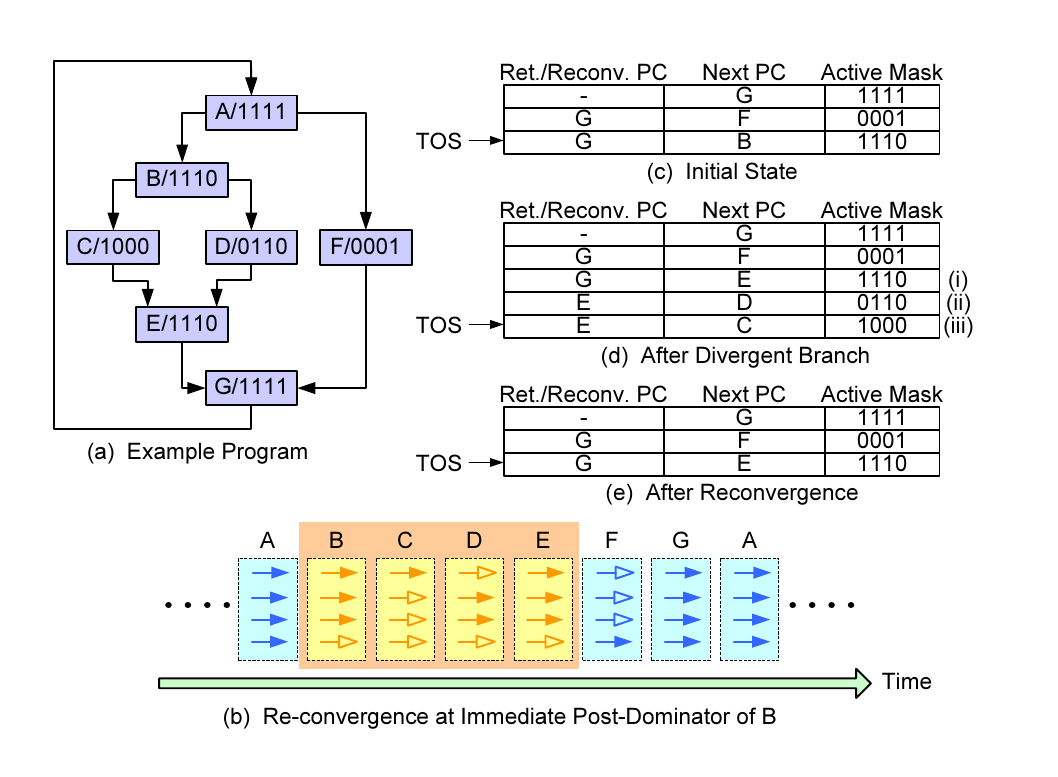
\includegraphics[scale=.45]{branch-re}
\end{figure}

La figure~\ref{BRANCHE} illustre le mécanisme de convergence de threads proposé dans l'article. Dans cet exemple, figure~\ref{BRANCHE}(a), un warp de 4 threads divergent après l'exécution du block A. Les threads exécutants le block B divergent encore un fois en deux blocks C et D.
\\Dans ce cas il existe plusieurs opportunités pour faire converger les threads pour resynchroniser leur exécution.
Tous les threads doivent exécuter le block G, il s'agit donc d'un point de convergence.
De même, tous les threads exécutant B doivent exécuter E, il vont donc être resynchronisés à ce block.

Les figures~\ref{BRANCHE}(c,d,e) montrent comment il est possible d'implémenter ce mécanisme grâce à une pile. Chaque élément de la pile est un triplet contenant le prochain PC (programme counter), le PC de convergence et un masque d'exécution indiquant quels threads sont concernés par l'entrée.
Dans l'exemple, lors de la détection du branchement à B, la tête de la pile (TOS) est mise à jour pour prendre en compte le nouveau point de convergence E. Les deux branches C et D sont ajoutées en tête de pile.


Pour déterminer le point de convergence des threads, les auteurs de cet article propose d'utiliser un concept issu de la compilation : l'\emph{immediate post-dominator}. Un block X est \emph{post-dominator} d'un block Y si tous les chemins d'exécution de Y vers le block de sortie passent par X. X est un \emph{immediate post-dominator} de Y s'il n'existe aucun \emph{post-dominator} de Y ayant pour \emph{post-dominator} X.
Les \emph{post-dominator} sont déterminables de manière statique à la compilation.

La convergence de threads au \emph{immediate post-dominator} permet un gain de performance significatif par rapport à une implémentation naïve des branchements sur une architecture SIMD.
Sur la figure~\ref{IPC}, on peut observer que l'implémentation naïve obtient 20\% des performances d'une machine MIMD d'IPC maximal équivalent et que l'implémentation avec convergence au post-dominator immédiat (PDOM) obtient lui 60\% de l'IPC de la machine MIMD.
Cette solution, relativement simple à implémenter, permet donc un fort gain d'efficacité sur la gestion des branchements sur les architectures SIMD.

On observe malgré tout que la machine MIMD reste beaucoup plus performante, les auteurs de l'article proposent donc d'autres mécanismes pour améliorer encore la gestion des branchements.

\subsection{Formation dynamique de warps}

Malgré l'utilisation du mécanisme de convergence, on a donc une utilisation sous-optimale de le pipeline SIMD lors d'exécution de branchements divergeant. Lors de l'exécution d'un seul warp de threads sur le pipeline SIMD, il est malheureusement impossible d'améliorer l'utilisation du matériel.
Dans la plupart des cas cependant, plusieurs warps exécutent le même programme en même temps.
Les auteurs de l'article proposent donc d'exploiter cette situation en groupant dynamiquement, à l'exécution, les threads de warps différents exécutant le même flux de contrôle.

Leur solution consiste à dynamiquement créer de nouveaux warps pour regrouper ensemble les threads exécutant le même flux de contrôle afin d'avoir un maximum de threads s'exécutant en même temps sur le pipeline SIMD.

\begin{figure}[h]
   \caption{\label{FUSION} Exemple de formation dynamique de warps}
   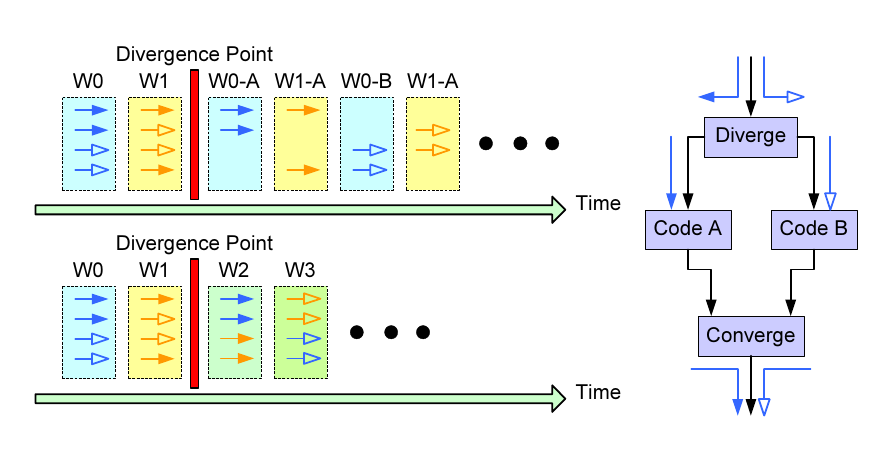
\includegraphics[scale=.5]{fusion}
\end{figure}

Sur l'exemple figure~\ref{FUSION} deux warps de 4 threads, W0 et W1, exécutent le même code dans lequel se trouve un branchement.
Sur le graphique, les flèches pleines divergent vers le block A et les flèches blanches divergent vers le block B.
Le cycle d'exécution du haut correspond à une exécution sans formation dynamique de warps, et celle du bas avec formation dynamique de warps.
Dans ce cas idéal, deux threads de chaque blocks exécutent A et B, il suffit donc de regrouper ensemble les threads exécutant A dans un nouveau warp W2 et les threads exécutant B dans un nouveau warp W3.
Ainsi, au lieu d'avoir quatre exécution de blocks avec seulement la moitié du pipeline SIMD utilisée, on l'utilise pleinement grâce aux nouveaux warps formés.

L'article propose que à chaque cycle, le scheduler de threads essaye de former de nouveaux warps de threads à partir des threads disponibles possédant le même PC suivant.

Ce mécanisme peut sembler idéal, cependant quelques problèmes émergent pour lesquels les auteurs de l'article proposent des solutions.

La création de nouveaux warps de threads implique qu'un thread peut potentiellement s'exécuter sur n'importe quelle ligne scalaire du pipeline SIMD, imposant que tous les registres soit accessibles de n'importe quelle de ces lignes. Or, le plus souvent, chaque ligne scalaire à accès à une \emph{bank} de registre.
Pour que tout les threads aient accès à tous les registres, il serait nécessaire d'implémenter un réseau d'interconnexion en \emph{crossbar}, et malgré cela, si plusieurs threads tentent d'accéder à la même bank, cela créé un conflit bloquant le pipeline.

Cette solution n'est donc pas réaliste, au lieu d'utiliser cela, les auteurs de l'article proposent de réunir au sein d'un nouveau warp uniquement des threads utilisant des bank de registres différentes. 
Dans certains cas, les auteurs notent qu'il peut ne pas être possible de créer des warps plus grands que initialement à cause de cette limitation.
Les expérimentations montrent cependant que cette solution a des performances proches de ce qu'on obtiendrait dans un cas idéal sans conflit de bank.

\subsection{Politique d'ordonnancement}

Pour que la formation dynamique de warps soit efficace, il faut qu'un grands nombre de threads aient le même PC au même moment. Si ce n'est pas le cas, le scheduler ne pourra pas regrouper des threads au sein d'un même warp.
Les auteurs de l'article ont essayer plusieurs politique d'ordonnancement, celle qu'ils ont retenu consiste à exécuter en priorité les warps ayant le PC majoritaire avant de choisir un nouveau PC. Les expérimentation montrent que ce choix est en général assez performant.
Cependant, le choix d'une heuristique pour l'ordonnancement nécessiterait un travail plus approfondi qui n'entre pas dans le cadre de l'article.

\section{Conclusion}

Dans cet article, les auteurs montrent qu'avec la démocratisation de l'utilisation de GPUs pour du calcul généraliste, l'inefficacité des architectures SIMD des GPUs à gérer les branchements est devenue problématique.
Dans leur articles ils proposent diverse amélioration architecturales permettant de grandement améliorer les performances dans des programmes contenant des branchements.

Depuis la publication de cet article, l'utilisation de GPUs pour du calcul généraliste a fortement augmenté, un grand nombre de super-calculateur du TOP500 utilisent des GPUs.
A l'heure actuelle, les GPUs sont énormément utilisés pour du calcul, avec notamment la démocratisation du \emph{Deep Learning} et des \emph{cryptomonnaies}. 

Les architectures GPUs actuelles sont devenues beaucoup plus flexibles et orientées pour le calcul généraliste qu'à l'époque de la publication de l'article, mais restent toujours fondamentalement des architectures SIMD.
Cela montre l'intérêt important des travaux présentés dans l'article, puisque que les problématiques étudiées sont toujours d'actualité.

\end{document} 
